% !TeX encoding = UTF-8
% !TeX spellcheck = it_IT
% !TeX root = MatDiz.tex
\chapter{B}
\vspace{5mm} 
\lemma{baricentro}Punto in cui può essere concentrato tutto il peso di un corpo.\llemma{b. triangolo}In un triangolo punto d'incontro delle mediane\pointsto~\seeentry{mediana}.
\lemma{base}\titolettoa{In un sistema di numerazione}, numero di cifre, compreso lo zero, che servono ad rappresentare un numero.\titolettoa{Base potenza} nelle potenze, rappresenta il numero che deve essere moltiplicato per se stesso tante volte che è indicato dall'indice.\titolettoa{Base logarimo} Numero che ha per esponente il logaritmo\pointsto~\vedilemma{logaritmo} in modo da ottenere l'argomento.
\begin{figure}
	\centering
	\scaptionb{George Boole 1815-1864}
	\label{fig:georgeboolecolor}\floatfoot{Source: Di Haks-\url{http://www.enezeus.com/blog/wp-content/uploads/2006/10/hacker1.jpg}, Pubblico dominio,\url{https://commons.wikimedia.org/w/index.php?curid=1597609}}
	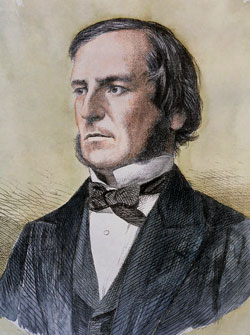
\includegraphics[width=0.7\linewidth]{Figure/B/George_Boole_color}
\end{figure}
\lemma{Bernoulli Daniel}\index{Bernoulli Daniel}(1700-1782) Nato a Groninga in Olanda il 29 gennaio 1700. Era figlio di Johann Bernoulli, nipote di Jacob Bernoulli, fratello più giovane di Nicolaus II Bernoulli, fratello più anziano di Johann II Bernoulli. Ha avuto pessimi rapporti con il padre anche lui matematico. Grande amico di Eulero\pointsto~\seeentry{Euler Leonard}\cite{Kline1972}
\begin{figure}
	\centering\scaptionb{Bernoulli Daniel 1700-1782}
	\label{fig:339px-eth-bib-bernoullidaniel1700-1782-portrait-portr10971}
	\floatfoot{By Unbekannt - E-Pics Bildarchiv online \url{http://doi.org/10.3932/ethz-a-000046381} \selectlanguage{english}{This image is from the collection of the ETH-Bibliothek and has been published on Wikimedia Commons as part of a cooperation with Wikimedia CH. Corrections and additional information are welcome. Public Domain,} \url{https://commons.wikimedia.org/w/index.php?curid=59419205}}
	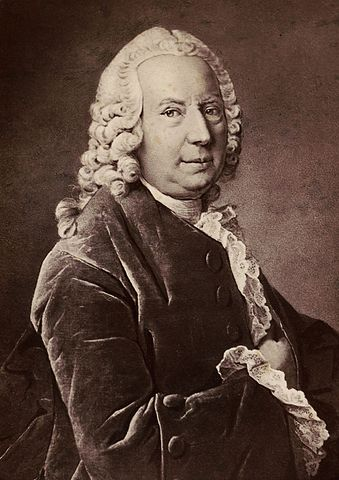
\includegraphics[width=0.7\linewidth]{Figure/B/Bernoulli_Daniel}
\end{figure}
\lemma{Bernoulli Jakob}(1654-1705) Fratello maggiore di Johann Bernoulli e zio di Daniel Bernoulli. Contribui allo sviluppo del calcolo infinitesimale. Tenne una corrispondenza con Gottfried Wilhelm von Leibniz\pointsto~\seeentry{Leibniz Gottfried Wilhelm}, uno dei fondatori del calcolo. La sua opera principale \textit{Ars Conjectandi}, pubblicata postuma nel 1713, contiene i fondamenti del calcolo delle probabilità.\index{Bernoulli Jakob}
\begin{figure}
\centering\scaptionb{Jakob Bernoulli (1654-1705)}
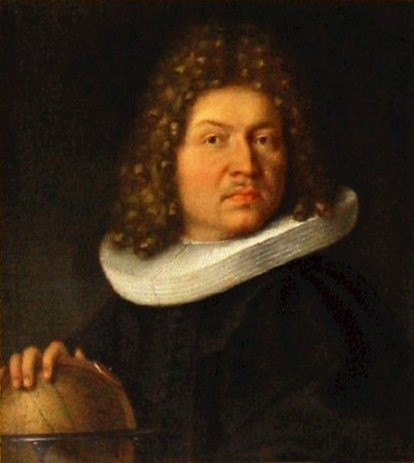
\includegraphics[width=0.7\linewidth]{Figure/B/Jakob_Bernoulli}
		\label{fig:jakobbernoulli}
\end{figure}
\lemma{Bernoulli Johann}\cite{Kline1972}\index{Bernoulli Johann}(1667-1748) Fratello di Jakob, fu allievo come lui di Leibniz\pointsto~\seeentry{Leibniz Gottfried Wilhelm}. contribui allo sviluppo del calcolo infinitesimale. Ebbe come allievo Eulero\pointsto~\seeentry{Euler Leonard}. Ebbe una controversia con Guillaume de l'Hopital  \pointsto~\vedilemma[Hopital Guillaume marchese de l']{Hôpital Guillaume marchese de l'}\ per l'omonima regola delle forme indeterminate.\index{Euler Leonard}
\begin{figure}
	\centering
\scaptionb{Johann I Bernoulli (1667-1748)}
	\label{fig:johannbernoulli}
	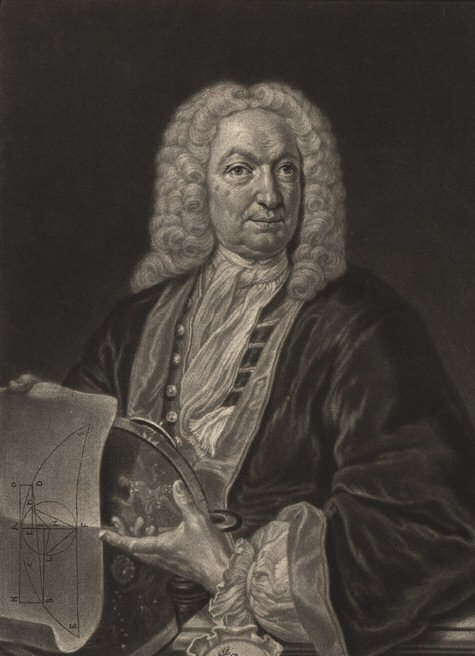
\includegraphics[width=0.7\linewidth]{Figure/B/Johann_Bernoulli}
\floatfoot{Di Johann Jakob Haid - Pubblico dominio, \url{https://commons.wikimedia.org/w/index.php?curid=57070}}
\end{figure}
\lemma{Bernoulli Nikolaus I}(1687-1759) Uno dei più importanti membri della famiglia Bernoulli. Era nipote di Jakob e Johann Bernoulli. Lavorò sulle equazioni differenziali e sulla geometria.
 \index{Bernoulli Nikolaus I}
 \lemma{Bernoulli Nikolaus II}(1695-1726) Fratello di Daniel Bernoulli. Contemporaneo di Eulero\pointsto~\seeentry{Euler Leonard} si trasferì a San Pietroburgo dove morì nel 1726. Successivamente la sua cattedra fu assegnata ad Eulero. 
 \cite{Kline1972}\index{Bernoulli Nikolaus II}
 \begin{figure}
 	\centering	\scaptionb{Nicolaus II Bernoulli (1695-1726)}
 	\label{fig:bernoullinicolausii}
 	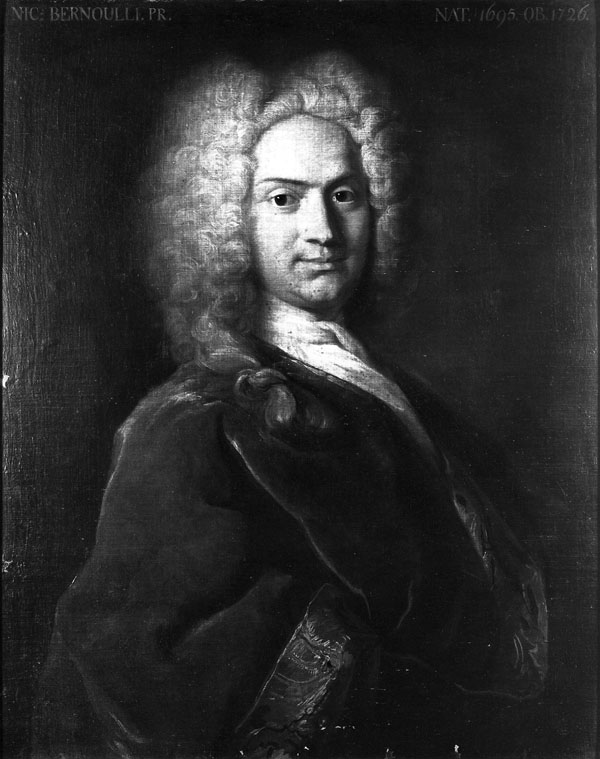
\includegraphics[width=0.7\linewidth]{Figure/B/Bernoulli_Nicolaussecondo}
 	\floatfoot{Di Johann Rudolf Huber - \url{http://www.simout.com/nicolaus-copernicus&page=327 } \url{https://commons.wikimedia.org/w/index.php?curid=10963524}}
  \end{figure}
\lemma{binario sistema}Sistema numerico a base due che usa le cifre \num{0} e \num{1} per rappresentare un numero.
\lemma{bisettrice}In un angolo\pointsto~\vedilemma{angolo}, semiretta\pointsto~\vedilemma{semiretta} con origine nel vertice, che divide l'angolo\pointsto~\vedilemma{angolo} in due parti uguali.
\lemma[Bolyai Janos]{Bolyai János}(1802-1860) Il suo contributo maggiore fu il suo lavoro nelle geometrie non euclidee.\index{Bolyai János}
\begin{figure}
	\centering
	\scaptionb[Janos Bolyai(1802 1860)]{János Bolyai(1802 1860)}
	\label{fig:bolyaijanosmarkosferencfestmenye}
	\floatfoot{Source: By Ferenc Márkos - Transferred from hu.wikipedia to Commons by Tambo., CC BY-SA 3.0, \url{https://commons.wikimedia.org/w/index.php?curid=24338736}}
	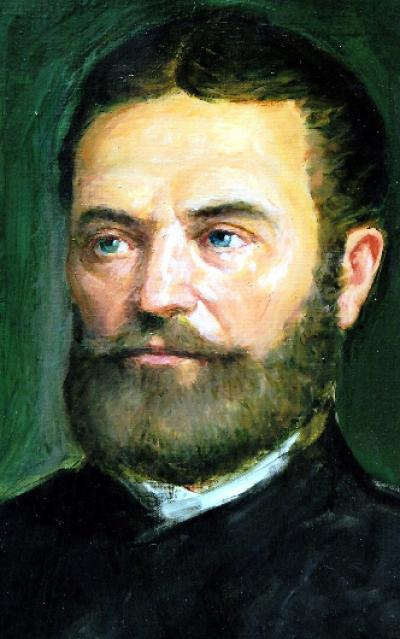
\includegraphics[width=0.7\linewidth]{Figure/B/Bolyai_Janos}
\end{figure}
\lemma{Bombelli Raffaele}\index{Bombelli Raffaele}(1526- ? 1572ca) Matematico e ingegnere diede una definizione chiara dei numeri negativi. Prese in considerazione i complessi nella risoluzione delle equazioni cubiche. Definì in termini moderni le quattro operazioni con i numeri complessi\vedilemma{n. complesso} anche se, non li accettava completamente (\textit{Algebra} 1572) \cite{Kline1972}.
\lemma{Bool George} (1815-1864)\index{Bool George}  nato a Lincoln il due novembre 1815 da un'umile famiglia. Nel 1854 pubblicò <<\textit{Indagine sulle leggi del pensiero}>>. Questo libro è alla base dell'algebra booleana. Il 24 novembre 1864 muore a Cork.\cite{Nahin2015} 
\lemma{Briggs Henry}(1561-1630)Scrisse la prima tabella dei logaritmi in base dieci \cite{Kline1972} nel 1617. Nel 1624  pubblicò \textit{Arithmetica logarithmica} ampliando tale tabella \cite{Boyer1980}.
\lemma{byte} Otto bit.